\documentclass[a4paper]{article}

\usepackage{babel}
\usepackage[latin1]{inputenc}
\usepackage{amssymb}
\usepackage{framed}
\usepackage{graphicx}
\usepackage{subcaption}

\setlength{\parindent}{0pt}
\setlength{\parskip}{3ex}

\begin{document}

\begin{center}
  {\large Artificial Neural Networks and Deep Architectures, DD2437}\\
  \vspace{7mm}
  {\huge Short report on lab assignment 2\\[1ex]}
  {\Large Radial basis functions, competitive learning and self-organisation}\\
  \vspace{8mm}  
  {\Large Rakin Ali, Steinar Logi and Hasan Alzubeidi}\\
  \vspace{4mm}
  {\large February, 08 2023\\}
\end{center}

\section{Main objectives and scope of the assignment}

Our major goals in the assignment were  
\begin{itemize}
\item To build, design and analyze a RBF network 
\item To understand Vector Quantization and how to implement it  
\item To implement Self-organising maps in order to understand the underlying theory behind it
\end{itemize}
In order to gain better theoretical foundations on how these models work, situations on when to use them and understand how to build them.

\section{Methods} All parts of the labs were implemented twice just to be safe. Everything was written in Python 3.9 and all plots were done with Matplotlib. 
\section{Results on RBF networks}
\textbf{3.1 Function approximation with RBF networks:} We approximated $sin(2x)$ and $square(2x)$ functions using RBF networks, achieving low error rates with minimal units. For the sine function, placing units at strategic points (minima, maxima, interval ends) proved effective. For the square function, employing the $sgn(y)$ activation function eliminated errors. The radial basis functions had a width of 2. Figures omitted to stay within 6 pages.

\textbf{3.2 Function approximation with noisy data:}
Here several tests were conducted to approximate $sin(2x)$ and $square(2x)$ containing noise on the training and test set to see how RBF networks perform, testing different parameters and comparing delta rule against least square rule.

\begin{figure}[ht]
    \centering
    \begin{subfigure}{0.4\textwidth}
        \centering
        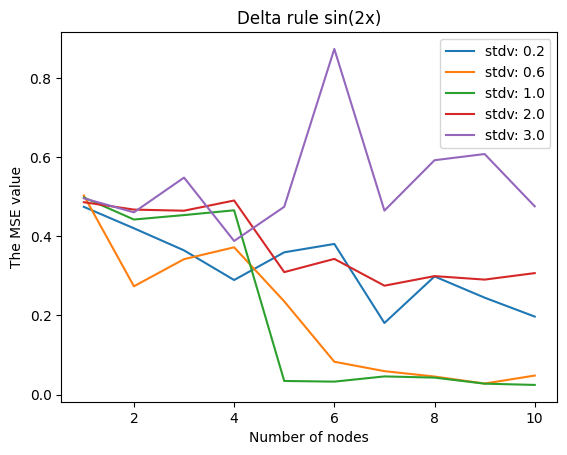
\includegraphics[width=\textwidth]{Labs/Lab 2/figures/3.2/MSE_sin(2x)_delta.png}
        \caption{Delta rule}
    \end{subfigure}
    \hfill
    \begin{subfigure}{0.4\textwidth}
        \centering
        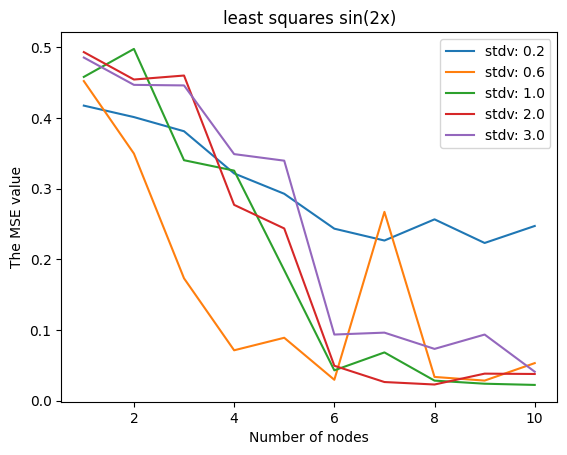
\includegraphics[width=\textwidth]{Labs/Lab 2/figures/3.2/MSE_sin(2x)_least.png}
        \caption{Least square}
    \end{subfigure}
    \hfill
    \caption{The MSE error with different in different BRF network}
    \label{fig:different-widths-units}
\end{figure}

As expected the MSE error decreases when the number of units increases except when the width is too low for the least square approach. The same pattern is seen in sequential learning when the width is 0.6 and 1. However, the number of units does not affect the performance when the width is too low or larger than one. See Figure \ref{fig:different-widths-units}. Learning constant is was crucial in training RBF networks. Large networks jumps the minima while small learning rate requires more epochs to converge. Images purposefully omitted to stay within 6 pages

We also compared two methods to choose the positions of the RBF nodes: the random and the shifted approach. It seems that the performance of the least square method is not affected by how we choose the positions of nodes. The methods give more or less the same result. However, sequential learning induces better performance when the shifted weights are picked. See Figure \ref{fig:Random weights}

\begin{figure}[htb]
    \centering
    \begin{subfigure}{0.4\textwidth}
        \centering
        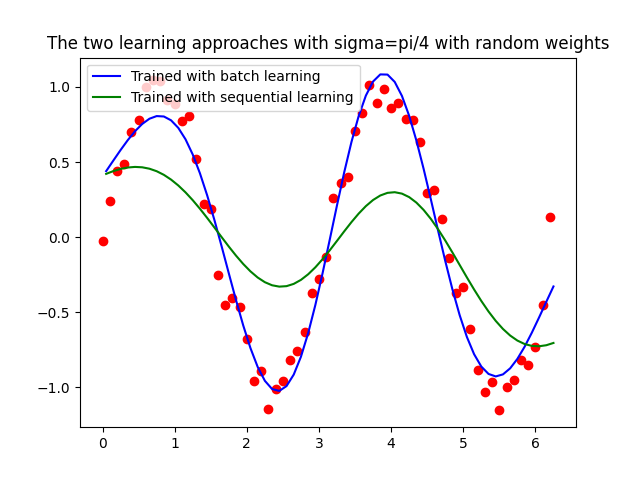
\includegraphics[width=\textwidth]{Labs/Lab 2/Steinar/results/comparison-random-weights.png}
        \caption{random-weights}
    \end{subfigure}
    \hfill
    \begin{subfigure}{0.4\textwidth}
        \centering
        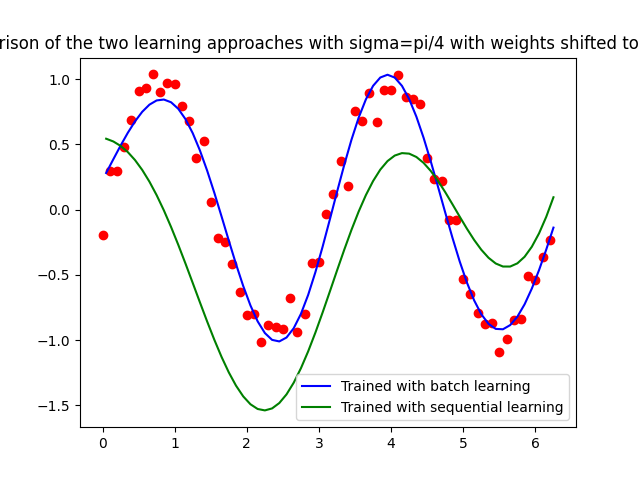
\includegraphics[width=\textwidth]{Labs/Lab 2/Steinar/results/comparison-weights-shifted.png}
        \caption{weights-shifted}
    \end{subfigure}
    \hfill
    \caption{Comparison of the random and shifted method}
    \label{fig:Random weights}
\end{figure}

When comparing a Perceptron network with a single hidden layer with the RBF network with the same amount of hidden nodes, the results indicate that RBF has a better performance and generalization. In Figure \ref{fig:comp-BRF-perc} we compared 10000 nodes in the Perceptron versus 7 nodes in the RBF network with the same dataset.
\begin{figure}[ht]
    \centering
    \begin{subfigure}{0.4\textwidth}
        \centering
        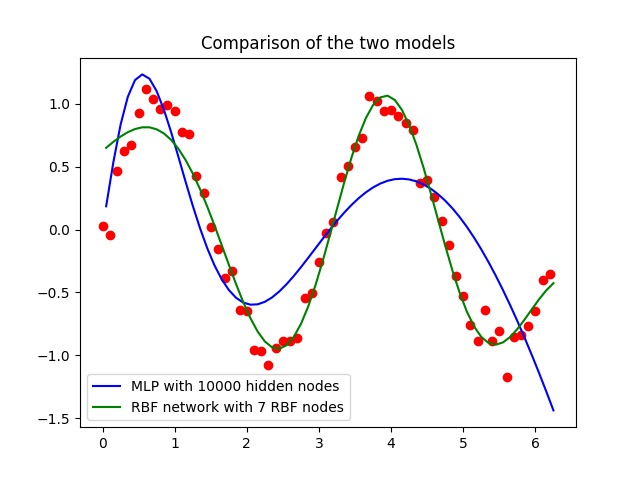
\includegraphics[width=\textwidth]{Labs/Lab 2/10000.jpg}
        \caption{10000 neurons}
    \end{subfigure}
    \hfill
    \begin{subfigure}{0.4\textwidth}
        \centering
        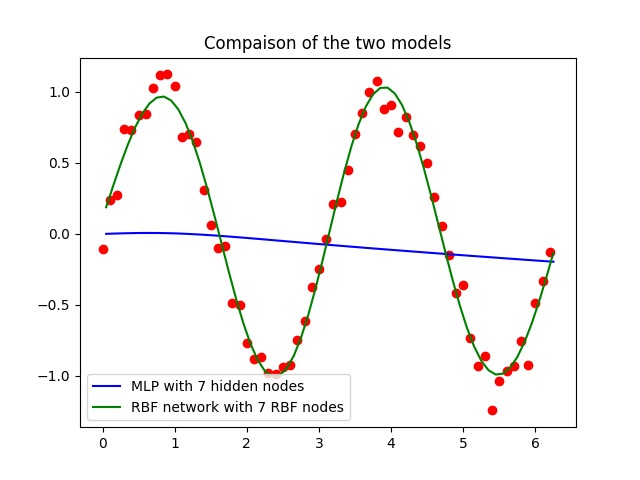
\includegraphics[width=\textwidth]{Labs/Lab 2/77.jpg}
        \caption{7 neurons}
    \end{subfigure}
    \hfill
    \caption{Comparison of the RBF network and perceptron network }
    \label{fig:comp-BRF-perc}
\end{figure}

Lastly we tested the model on a clean test set however trainde on the noisy dataset. Teh results showed good generalization. Illustration of the predictions can seen in Figure \ref{fig:performance-clean}  

\begin{figure}[htb]
    \centering
    \begin{subfigure}{0.4\textwidth}
        \centering
        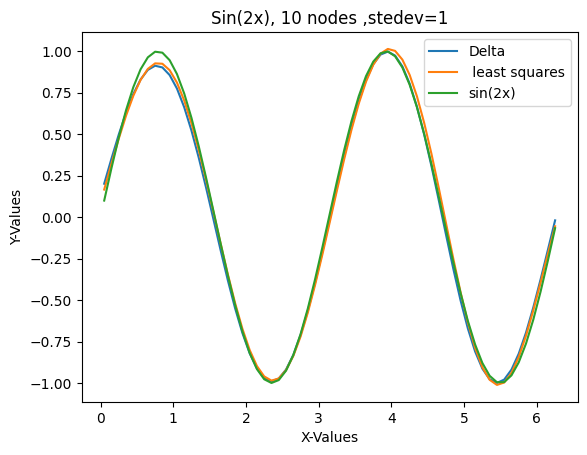
\includegraphics[width=\textwidth]{Labs/Lab 2/figures/3.2/Performance_sin(2x)_clean.png}
        \caption{Sin(2x)}
    \end{subfigure}
    \hfill
    \begin{subfigure}{0.4\textwidth}
        \centering
        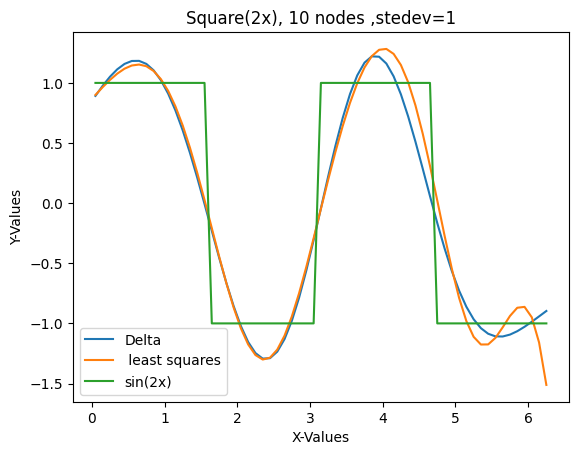
\includegraphics[width=\textwidth]{Labs/Lab 2/figures/3.2/performance_square(2x)_clean.png}
        \caption{square(2x)}
    \end{subfigure}
    \hfill
    \caption{The prediction of the clean data}
    \label{fig:performance-clean}
\end{figure}

\textbf{3.3 Competitive learning for RBF unit initialisation} In this part of the assignment we used competitive learning to initialize the weights used in the RBF network that was trained on the training set from the $sin(2x)$ function.

The results can be seen in figure \ref{fig:cl}. The image on the left shows the function approximation on the dataset without noise and the right with noise on the function. On both images the weights obtained from the competitive learning can be seen as the orange dots on the x-axis. The width of the rbf nodes was the number of weights divided by the domain of the function or $2\pi$ in both cases. 

When we tried this using 6 nodes we obtained a worse results than when we manually placed the weights in the weight space but still the results were accurace. The absolute relative error for the function with noise was around 0.104 so the network seems to generalize pretty well. 


\begin{figure}[ht]
    \centering
    \begin{subfigure}{0.4\textwidth}
        \centering
        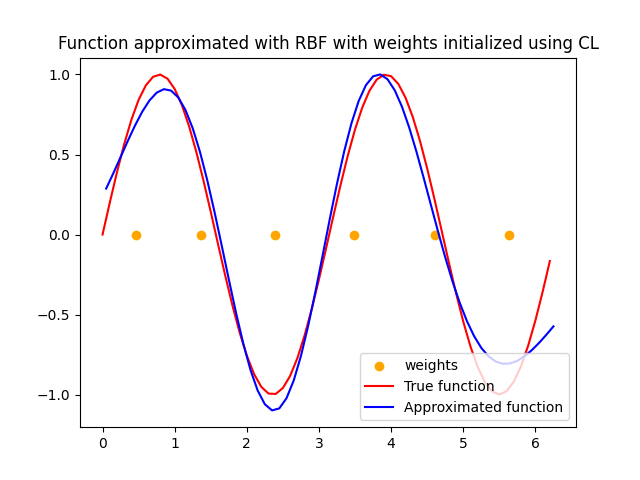
\includegraphics[width=\textwidth]{Labs/Lab 2/Steinar/results/no-noise-approx-cl.png}
    \end{subfigure}
    \hfill
    \begin{subfigure}{0.4\textwidth}
        \centering
        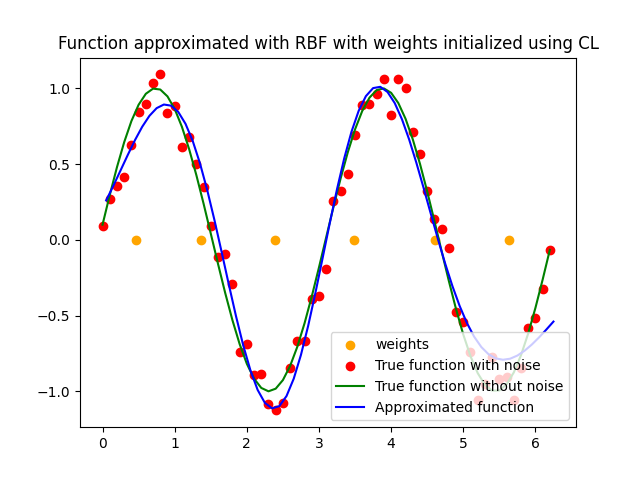
\includegraphics[width=\textwidth]{Labs/Lab 2/Steinar/results/noise-function-cl.png}
    \end{subfigure}
    \caption{RBF networks with weights initialized using CL}
    \label{fig:cl}
\end{figure}

As can be seen in these images in figure \ref{fig:cl} the weights are evenly rather evenly spaced on the x-axis. This makes sense since there are no clusters in the input space. The input data is evenly distributed on the x-axis and therefore the weights are evenly distributed on the x-axis.

\textbf{3.4 CL to initialize RBF units with 2-dimensional input}
We used an RBF network to approximate a two dimensional function with two dimensional output. The dataset provided was the \textit{ballist} data set and a test dataset, \textit{balltest}. We used competitive learning to initialize the RBF weights. The RBF network proved to be pretty good at approximating this function. A picture of the weights found by competitive learning can be seen in figure \ref{fig:cl-2-dim} where they are plotted in the input space. We tested this with a different number of nodes and found that using 10 RBF nodes gave us pretty good results that generalized well. The mean square error on the test set was 0.0124 and the mean square error on the train set was 0.0066.

\begin{figure}[ht]
    \centering
    \begin{subfigure}{0.4\textwidth}
        \centering
        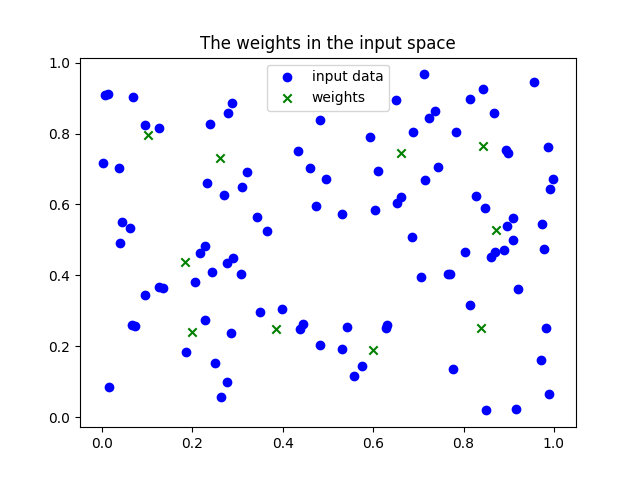
\includegraphics[width=\textwidth]{Labs/Lab 2/Steinar/results/weights-cl.png}
    \end{subfigure}
    \hfill
    \begin{subfigure}{0.4\textwidth}
        \centering
        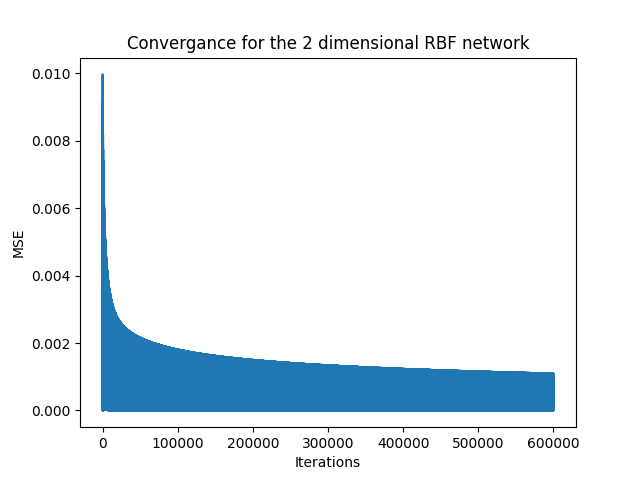
\includegraphics[width=\textwidth]{Labs/Lab 2/Steinar/results/2-dim-convergance.png}
    \end{subfigure}
    \caption{The weight positions in the input space}
    \label{fig:cl-2-dim}
\end{figure}


\section{Results on SOM netowrk}
\begin{figure} [htb]
    \centering
    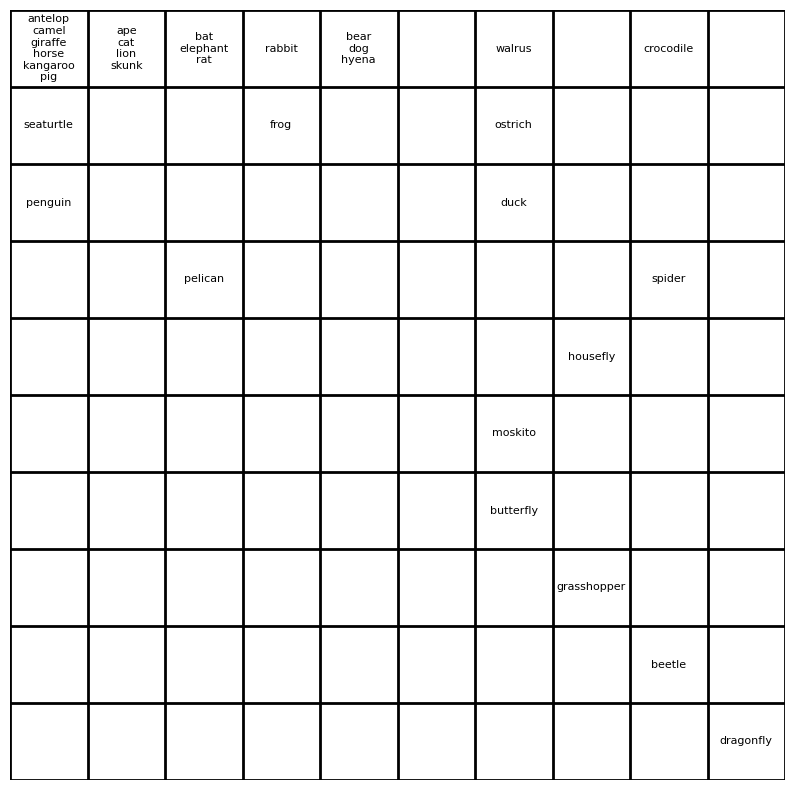
\includegraphics[width=5cm]{Labs/Lab 2/Results/animal_som.png}
    \caption{Animals sorted in 100 size nodes}
    \label{fig:SOM_animals}
\end{figure}
\textbf{4.1: SOM network of Animal dataset: } In the code we set the initial neighbors to 50, had 1000 epochs and a learning rate of 0.2 as in the instructions. The figure can be seen in \ref{fig:SOM_animals}. The figure makes sense as cat and lion are matched together and with closer observation you'll notice how most insects are grouped together. However they are certain places where it does not entirely make sense, specifically between frog, ape and walrus. In general it made sense. 



\textbf{4.2 Cyclic tour: }Figure \ref{fig:SOM_cycle} represents the shortest cycling tour which passes through all the cities based on their coordinates. We got different paths whenever we ran the code. The dotted lines represent which city is closest to that node as in certain times the nodes were placed between two cities.  
\begin{figure}[htb]
    \centering
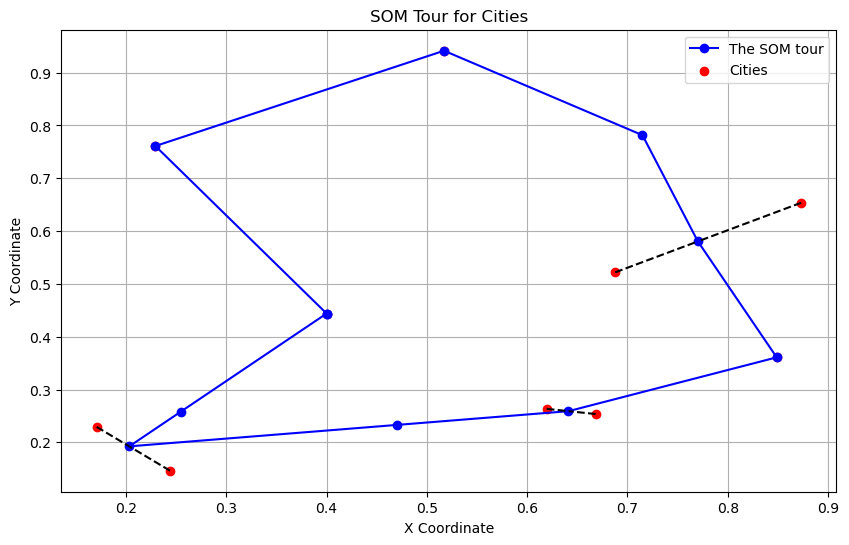
\includegraphics[width=7.5cm]{Labs/Lab 2/Results/Cyclic_som.png}
    \caption{Best path by SOM network}
    \label{fig:SOM_cycle}
\end{figure}

\textbf{4.3 Clustering with SOM}
\begin{figure}[htb]
    \centering
    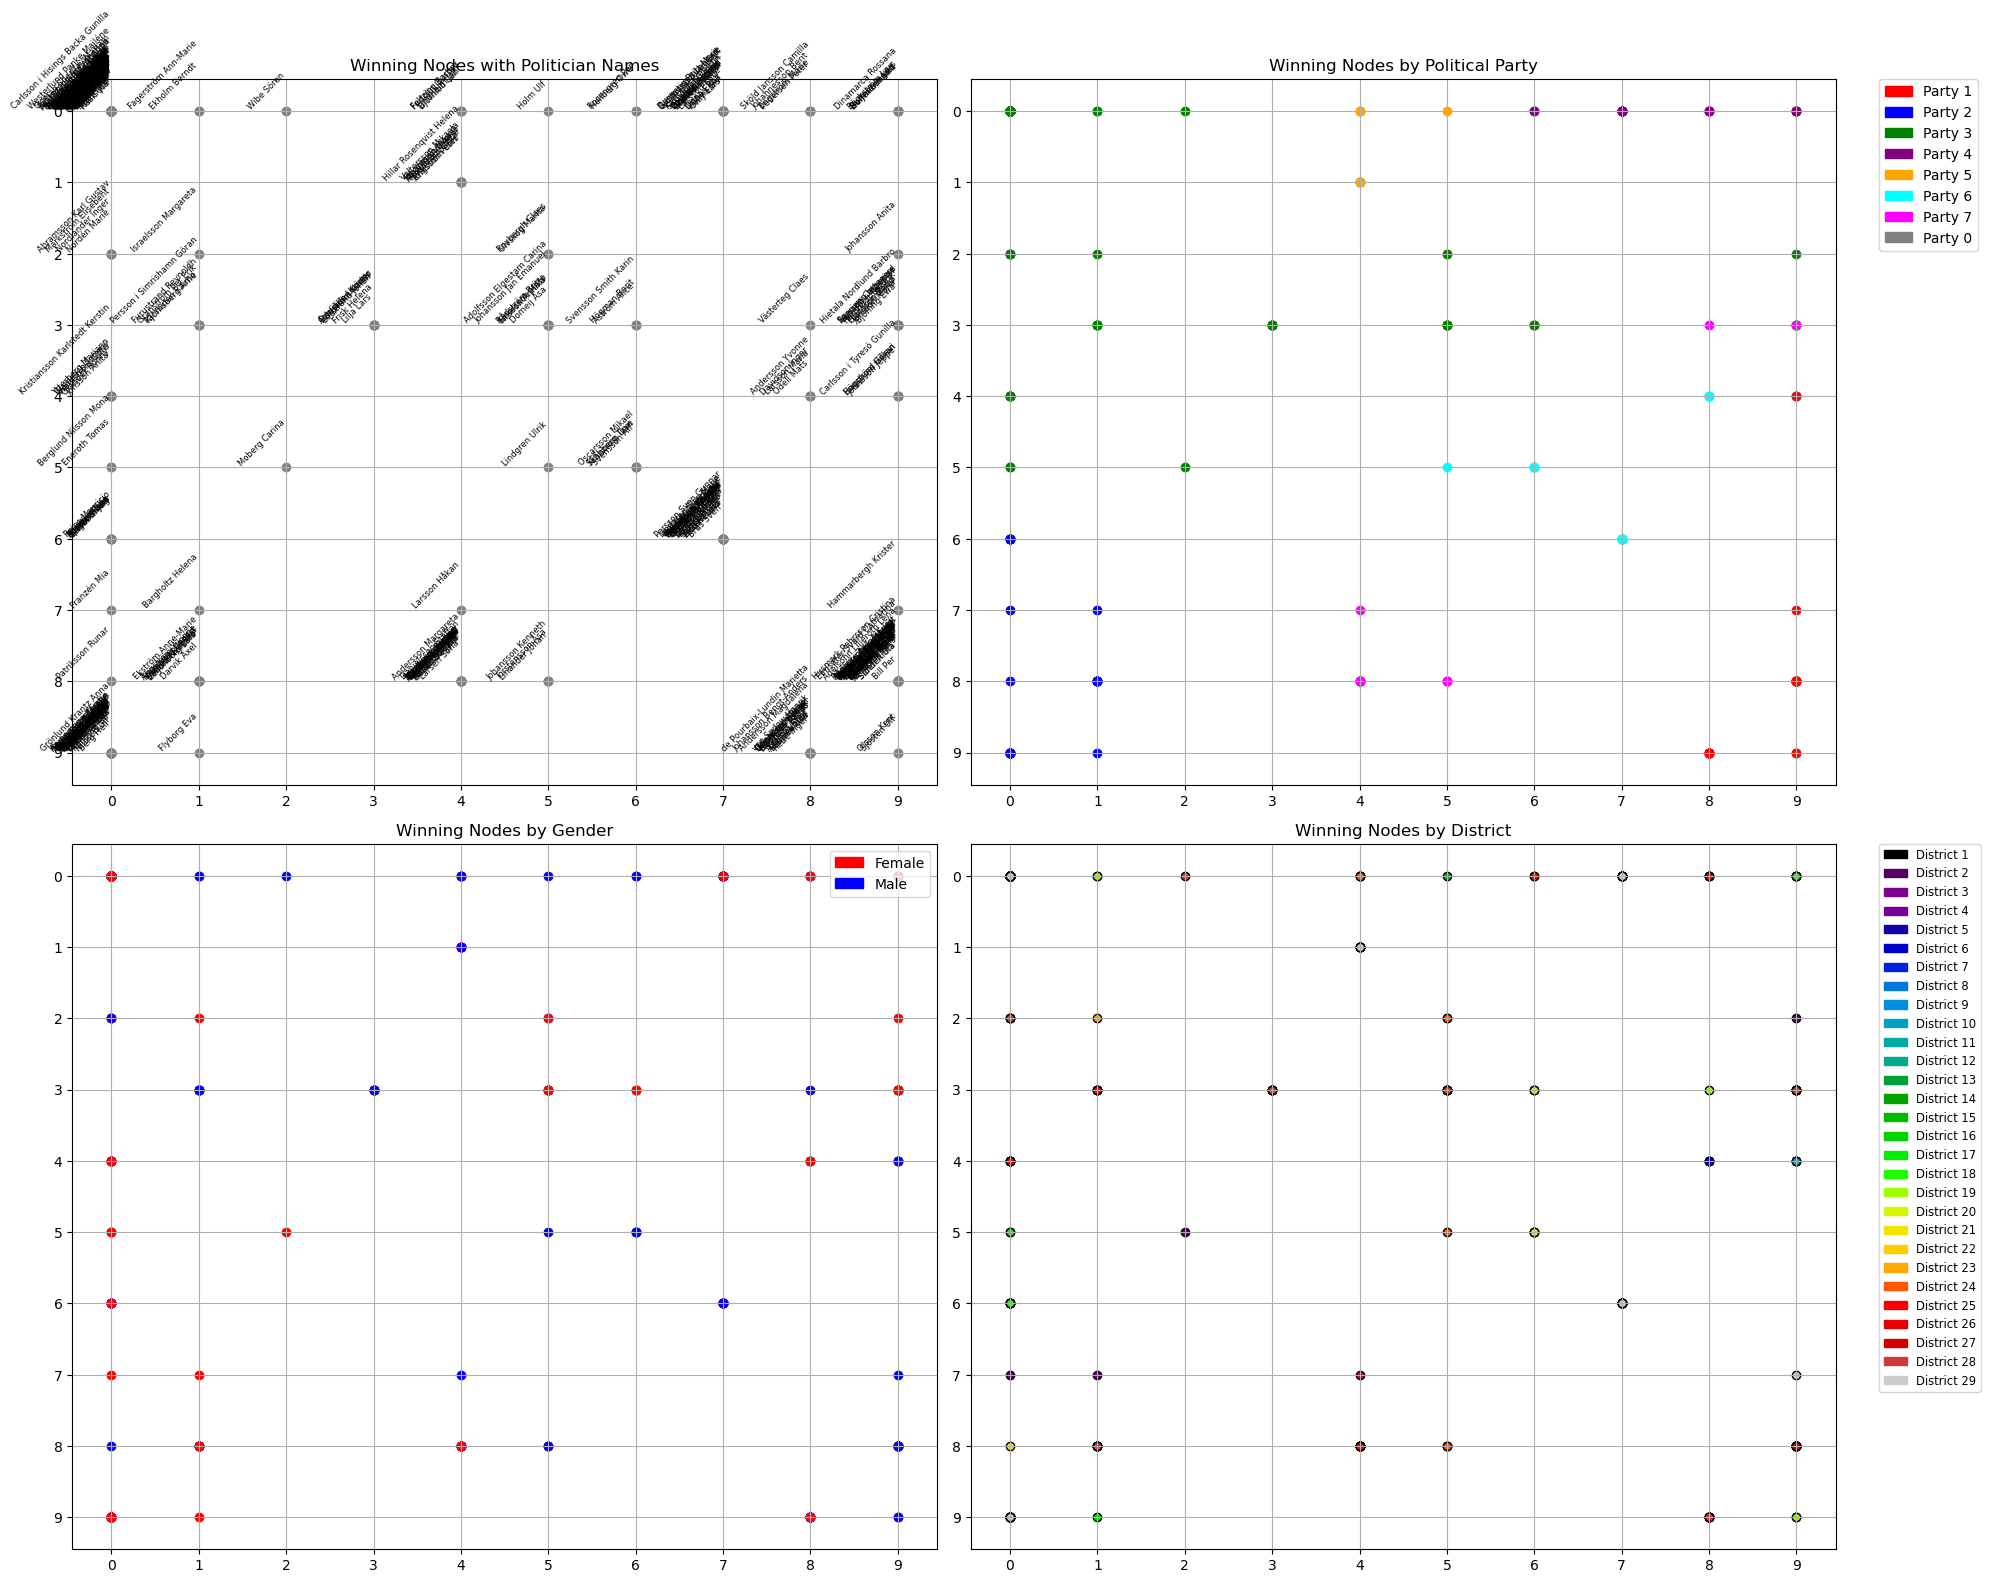
\includegraphics[width=9cm]{Labs/Lab 2/Results/politics_som.png}
    \caption{SOM grid based on political data}
    \label{fig:SOM_politics}
\end{figure}
In this assignment we were given a dataset on how 349 politicians voted on 31 separate decision and we were given their political party, gender, name and district. The results can be figure \ref{fig:SOM_politics}. In the subfigure at the top left, we to see the names of each 349 politicians and how similar they are to each other. On the figure to the top right, we see how similar each politician voted based on their political party and notice how closely most of them are to each other. The blue, red and green are tend to stick close to each together. Regarding district and gender, there is little there are no observable pattern. 




\section{Final remarks}
\begin{itemize}
    
    \item Zero error can be achieved to approximate the $square(2x)$ with use of $sgn(y)$
    
    
    \item Selecting strategic point positions such as minima, maxima can be effective to minimize the error. 
    
    \item Increasing the number of units with a good choice of width is sufficient to minimize the error and to achieve good generalization regardless of the positions of the units.
    
    \item The BRF network performs better than the perceptron with only one hidden layer, even if it consists of 10000 neurons.
    
    \item Choosing an appropriate number of neurons, width, and learning rate is crucial for good generalization. Good performance can be achieved, although the data are not clean. 
    
    \item SOM networks are somewhat good on finding patterns on the dataset and can be used a clustering algorithm. Get's difficult the more features the dataset hasl

    \item You cannot simply implement SOM network without understanding the underlying dataset. 
    

\end{itemize}

\end{document}
